\documentclass[tikz]{standalone}
    \usepackage{tikz}
    \usepackage{alphalph}
    \usetikzlibrary{positioning, graphs}
    \usetikzlibrary{graphs.standard}
    \begin{document}
    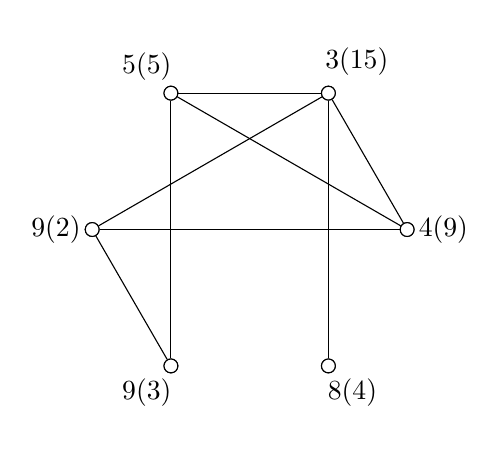
\begin{tikzpicture}
    \begin{scope}
        [every node/.style={draw,circle,inner sep = 0em, minimum size = 0.5em, fill = white},
        edgelabel/.style = {fill = white, inner sep = 0.1em, font=\small}]
       \graph[clockwise, radius = 2cm, phase = 0, empty nodes]{subgraph I_n[n = 6, name = A]};

       \node[label={0:$4(9)$}] (a) at (A 1) {};
       \node[label={300:$8(4)$}] (b) at (A 2) {};
       \node[label={240:$9(3)$}] (c) at (A 3) {};
       \node[label={180:$9(2)$}] (d) at (A 4) {};
       \node[label={120:$5(5)$}] (e) at (A 5) {};
       \node[label={60:$3(15)$}] (f) at (A 6) {};

       \draw[-] (A 1) to (A 4);
       \draw[-] (A 1) to (A 5);
       \draw[-] (A 1) to (A 6);
       \draw[-] (A 2) to (A 6);
       \draw[-] (A 3) to (A 4);
       \draw[-] (A 3) to (A 5);
       \draw[-] (A 4) to (A 6);
       \draw[-] (A 5) to (A 6);
            
    \end{scope}
    \end{tikzpicture}
    \end{document}